\documentclass{beamer}
\usepackage{amsmath,amssymb,tikz,graphicx,algorithmic,tabularx,lmodern}
%\includeonlyframes{show}
\usetikzlibrary{external}
\tikzexternalize[prefix=tikz/] % so that i don't have to compile the tikz pictures multiple times, run with pdflatex -shell-escape LLL.tex as latex needs t write new files
\newcommand{\scite}[1]{$\!^{\cite{#1}}$}
\newcommand\scalemath[2]{\scalebox{#1}{\mbox{\ensuremath{\displaystyle #2}}}}
\newcommand{\vabs}[1]{\left|\left|#1\right|\right|}
\newcommand{\bv}{\mathbf b}
\title{LLL algorithm and usage in cryptography}
\institute{libgen/scihub}
\author{Ariana}
\date{\today}
\usetheme{Singapore}
\addtobeamertemplate{navigation symbols}{}{%
	\usebeamerfont{footline}%
	\usebeamercolor[fg]{footline}%
	\hspace{1em}%
	\insertframenumber/\inserttotalframenumber
}
\begin{document}
	
\frame{\titlepage}

\begin{frame}
	\frametitle{Table of Contents}
	\begin{itemize}
		\item[-]Lattice reduction
		\item[]
		\item[-]Applications in algorithms
		\item[]
		\item[-]Cryptographic attacks
		\item[]
	\end{itemize}
\end{frame}

\section{Lattice reduction}

\begin{frame}
	\frametitle{Lattices}
    A lattice is a free $\mathbb Z$-module with $d$ generators as a subset of $\mathbb R^n$

    Example: $\mathbb Z^n$ in $\mathbb R^n$\pause

    A lattice reduction algorithm is an algorithm that finds a `short' and `nearly orthogonal' basis
\end{frame}

\begin{frame}
    \frametitle{Lattice in $\mathbb R^2$}
    \begin{center}
         \begin{tikzpicture}
            \draw(-4.5,0)--(4.5,0)(0,-3.5)--(0,3.5);
            \foreach\i in {-4,...,4}{
                \foreach[evaluate={
                        \x = \i+0.2*\j;
                        \y = \j-0.1*\i;
                        \tx = int(ceil(abs(\x)-0.5));
                        \ty = int(ceil(abs(\y)-0.4));
                    }]\j in {-4,...,4}{
                    \ifnum\tx<5
                    \ifnum\ty<4
                        \node[circle,fill=black,inner sep=0pt,minimum size=3pt]at(\x,\y){};
                    \fi
                    \fi
                }
            }
            \draw[->,color=red](0,0)--(2.6,2.8);
            \draw[->,color=red](0,0)--(-1.4,-1.9);
            \draw[->,color=black!30!green](0,0)--(1,-0.1);
            \draw[->,color=black!30!green](0,0)--(0.2,1);
        \end{tikzpicture} 
    \end{center}
\end{frame}

\begin{frame}
    \frametitle{Euclidean algorithm}
    The Euclidean algorithm returns the gcd of $a,b$

    \begin{algorithmic}
        \WHILE{$b\neq0$}
        \IF{$|a|>|b|$}
        \STATE $a,b\leftarrow b,a$
        \ENDIF
        \STATE $d\leftarrow\frac{b}{a}$
        \STATE $b\leftarrow b-\left\lfloor d\right\rceil a$
        \ENDWHILE
        \RETURN $a$
    \end{algorithmic}

    $a,b$ is just a lattice in $\mathbb R^1$ and $\gcd(a,b)$ is it's reduced lattice
\end{frame}

\begin{frame}
    \frametitle{Gaussian Lattice Reduction}
    Let $\bv_1,\bv_2$ be a basis

    \begin{algorithmic}
        \WHILE{$\left\lfloor\mu_{2,1}\right\rceil\neq0$}
        \IF{$\vabs{\bv_1}>\vabs{\bv_2}$}
        \STATE $\bv_1,\bv_2\leftarrow\bv_2,\bv_1$
        \ENDIF
        \STATE $\mu_{2,1}\leftarrow\frac{\left(\bv_2,\bv_1\right)}{\vabs{b_1}^2}$
        \STATE $\bv_2\leftarrow\bv_2-\left\lfloor\mu_{2,1}\right\rceil\bv_1$
        \ENDWHILE
        \RETURN $\bv_1,\bv_2$
    \end{algorithmic}
\end{frame}

\begin{frame}
    \frametitle{Example}
    \begin{center}
        \only<1-3>{\begin{tikzpicture}
            \draw(-4.5,0)--(4.5,0)(0,-3.5)--(0,3.5);
            \foreach\i in {-4,...,4}{
                \foreach[evaluate={
                        \x = \i+0.2*\j;
                        \y = \j-0.1*\i;
                        \tx = int(ceil(abs(\x)-0.5));
                        \ty = int(ceil(abs(\y)-0.4));
                    }]\j in {-4,...,4}{
                    \ifnum\tx<5
                    \ifnum\ty<4
                        \node[circle,fill=black,inner sep=0pt,minimum size=3pt]at(\x,\y){};
                    \fi
                    \fi
                }
            }
            \only<1>{
                \node at(2,3.5){$\mu_{2,1}=\frac{62}{39}$};
                \draw[->,color=blue,thick](0,0)--(-9/5, 6/5)node[anchor=south]{$\bv_1$};
                \draw[->,color=blue,thick](0,0)--(-13/5, 23/10)node[anchor=south west]{$\bv_2$};
                \draw[->,color=black,thick](0,0)--(17/65, 51/130);
                \draw[dotted,color=gray,thick](17/65, 51/130)--(-13/5, 23/10);
            }
            \only<2>{
                \node at(2,3.5){$\mu_{2,1}=\frac{-192}{101}$};
                \draw[->,color=blue,thick](0,0)--(1, -1/10)node[anchor=south]{$\bv_1$};
                \draw[->,color=blue,thick](0,0)--(-9/5, 6/5)node[anchor=south west]{$\bv_2$};
                \draw[->,color=black,thick](0,0)--(51/505, 102/101);
                \draw[dotted,color=gray,thick](51/505, 102/101)--(-9/5, 6/5);
            }
            \only<3>{
                \node at(2,3.5){$\mu_{2,1}=\frac{10}{101}$};
                \draw[->,color=blue,thick](0,0)--(1, -1/10)node[anchor=south]{$\bv_1$};
                \draw[->,color=blue,thick](0,0)--(1/5, 1)node[anchor=south west]{$\bv_2$};
                \draw[->,color=black,thick](0,0)--(51/505, 102/101);
                \draw[dotted,color=gray,thick](51/505, 102/101)--(1/5, 1);
            }
        \end{tikzpicture}}
    \end{center}
\end{frame}

\begin{frame}
    \frametitle{Gram-Schmidt}
    For some vectors $\bv_i\in\mathbb R^n$, define the orthogonal vectors $\bv^*_i$ as

    $$\bv^*_i=\bv_i-\sum_{j=1}^{i-1}\frac{\left(\bv_i,\bv^*_j\right)}{\vabs{\bv^*_j}^2}\bv^*_j=\bv_i-\sum_{j=1}^{i-1}\mu_{j,i}\bv^*_j$$

    with $\mu_{i,j}=\frac{\left(\bv_i,\bv^*_j\right)}{\vabs{\bv^*_j}^2}$

    Then the space generated by $b_i$ and $b^*_i$ are the same

    Typically we normalize the vectors but for lattice reduction purposes this is not done
\end{frame}

\begin{frame}
    \frametitle{LLL-reduced}
    For some basis $\bv_i$, let $\bv^*_i$ be the Gram-Schmidt orthogonalized basis. Then the basis is LLL-reduced for $\delta\in\left(\frac14,1\right)$ iff:\pause

    $$\mu_{i,j}=\frac{\left(\bv_i,\bv^*_j\right)}{\vabs{\bv^*_j}^2}$$

    \begin{enumerate}
        \item Size reduced: $j<i,\mu_{i,j}\leq\frac12$\pause
        \item Lov\'asz condition: $\left(\delta-\mu_{i+1,i}^2\right)\vabs{\bv^*_i}^2\leq\vabs{\bv^*_{i+1}}^2$
    \end{enumerate}
\end{frame}

\begin{frame}
    \frametitle{LLL algorithm}
    \begin{algorithmic}
        \STATE $i\leftarrow2$
        \WHILE{$i<n$}
            \FOR{$j=i-1,i-2,...,1$}
                \IF{$\left|\mu_{i,j}\right|>\frac12$}
                    \STATE $\bv_i\leftarrow\bv_i-\left\lfloor\mu_{i,j}\right\rceil\bv_j$
                \ENDIF
            \ENDFOR
            \IF{$\left(\delta-\mu_{i,i-1}^2\right)\vabs{\bv^*_{i-1}}^2\leq\vabs{\bv^*_i}^2$}
                \STATE $i\leftarrow i+1$
            \ELSE
                \STATE $i\leftarrow\max(i-1,2)$
                \STATE $\bv_{i-1},\bv_i\leftarrow\bv_i,\bv_{i-1}$
            \ENDIF
        \ENDWHILE
    \end{algorithmic}
\end{frame}

\begin{frame}
    \frametitle{Example}
    \begin{center}
        \begin{tabular}{*{3}{>{\centering\arraybackslash}p{0.25\textwidth}}}
            $\bv_1$&$\bv_2$&$\bv_3$\\
            $
            \only<1-7>{\left(1,2,0\right)}
            \only<8->{\left(1,0,1\right)}
            $&
            $
            \only<1>{\left(1,3,2\right)}
            \only<2-5>{\left(0,1,2\right)}
            \only<6-7>{\left(1,0,1\right)}
            \only<8-12>{\left(1,2,0\right)}
            \only<13->{\left(-1,1,1\right)}
            $&
            $
            \only<1-4>{\left(2,2,1\right)}
            \only<5>{\left(1,0,1\right)}
            \only<6-11>{\left(0,1,2\right)}
            \only<12>{\left(-1,1,1\right)}
            \only<13->{\left(1,2,0\right)}
            $\\[5mm]
            $\bv^*_1$&$\bv^*_2$&$\bv^*_3$\\
            $
            \only<1-7>{\left(1,2,0\right)}
            \only<8->{\left(1,0,1\right)}
            $&
            $
            \only<1-5>{\left(-\frac25,\frac15,2\right)}
            \only<6-7>{\left(\frac45,-\frac25,1\right)}
            \only<8-12>{\left(\frac12,2,-\frac12\right)}
            \only<13->{\left(-1,1,1\right)}
            $&
            $
            \only<1-5>{\left(\frac{20}{21},-\frac{10}{21},\frac5{21}\right)}
            \only<6-12>{\left(-\frac{10}9,-\frac59,\frac{10}9\right)}
            \only<13->{\left(\frac56,-\frac53,-\frac56\right)}
            $\\
        \end{tabular}
        $$
        \only<1>{\mu_{2,1}=\frac75}
        \only<2>{\mu_{2,1}=\frac25}
        \only<3>{\mu_{3,2}=\frac8{21}}
        \only<4>{\mu_{3,1}=\frac65}
        \only<5>{\mu_{3,2}=\frac8{21}}
        \only<6-7>{\mu_{2,1}=\frac15}
        \only<8-9>{\mu_{2,1}=\frac12}
        \only<10>{\mu_{3,2}=\frac29}
        \only<11>{\mu_{3,1}=1}
        \only<12>{\mu_{3,2}=\frac29}
        \only<13-14>{\mu_{2,1}=0}
        \only<15>{\mu_{3,2}=\frac13}
        \only<16>{\mu_{3,1}=\frac12}
        \only<17>{\mu_{3,1}=\frac12}
        $$
        $$
        \only<2>{\left(\frac34-\left(\frac25\right)^2\right)\vabs{\bv^*_1}^2\leq\vabs{\bv^*_2}^2}
        \only<5>{\left(\frac34-\left(\frac8{21}\right)^2\right)\vabs{\bv^*_2}^2>\vabs{\bv^*_3}^2}
        \only<7>{\left(\frac34-\left(\frac15\right)^2\right)\vabs{\bv^*_1}^2>\vabs{\bv^*_2}^2}
        \only<9>{\left(\frac34-\left(\frac12\right)^2\right)\vabs{\bv^*_1}^2\leq\vabs{\bv^*_2}^2}
        \only<12>{\left(\frac34-\left(\frac29\right)^2\right)\vabs{\bv^*_2}^2>\vabs{\bv^*_3}^2}
        \only<14>{\left(\frac34-\left(0\right)^2\right)\vabs{\bv^*_1}^2\leq\vabs{\bv^*_2}^2}
        \only<17>{\left(\frac34-\left(\frac12\right)^2\right)\vabs{\bv^*_2}^2\leq\vabs{\bv^*_3}^2}
        $$
    \end{center}
\end{frame}

\begin{frame}
    \frametitle{Example}
    $$\begin{pmatrix}
        1&2&0\\1&3&2\\2&2&1
    \end{pmatrix}\to
    \begin{pmatrix}
        1&0&1\\
        -1&1&1\\
        1&2&0
    \end{pmatrix}
    $$

    \begin{center}
    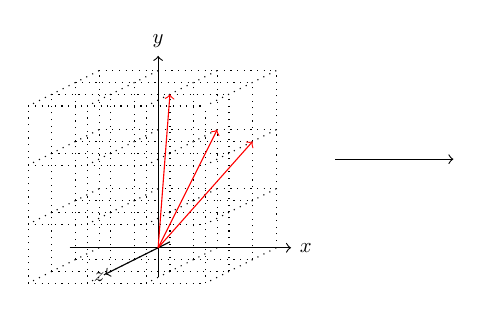
\begin{tikzpicture}[z={(-0.4,-0.2)},scale=0.75,every node/.style={transform shape}]
        \foreach\x in {-1,...,2}{
        \foreach\y in {0,...,3}{
        \foreach\z in {0,...,3}{
            \ifnum\x<2
                \draw[dotted](\x,\y,\z)--(\x+1,\y,\z);
            \fi
            \ifnum\y<3
                \draw[dotted](\x,\y,\z)--(\x,\y+1,\z);
            \fi
            \ifnum\z<3
                \draw[dotted](\x,\y,\z)--(\x,\y,\z+1);
            \fi
        }
        }
        }
        \node at(2.5,0,0){$x$};
        \node at(0,3.5,0){$y$};
        \node at(0,0,2.5){$z$};
        \draw[->](-1.5,0,0)--(2.25,0,0);
        \draw[->](0,-0.5,0)--(0,3.25,0);
        \draw[->](0,0,-0.5)--(0,0,2.25);
        \draw[->,color=red](0,0,0)--(1,2,0);
        \draw[->,color=red](0,0,0)--(1,3,2);
        \draw[->,color=red](0,0,0)--(2,2,1);
        \draw[->](3,1.5,0)--(5,1.5,0);
    \end{tikzpicture}
    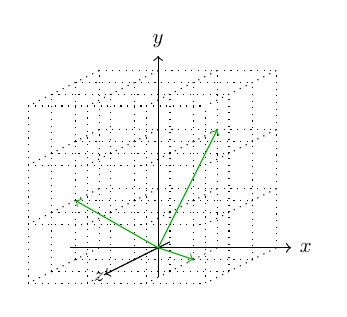
\begin{tikzpicture}[z={(-0.4,-0.2)},scale=0.75,every node/.style={transform shape}]
        \foreach\x in {-1,...,2}{
        \foreach\y in {0,...,3}{
        \foreach\z in {0,...,3}{
            \ifnum\x<2
                \draw[dotted](\x,\y,\z)--(\x+1,\y,\z);
            \fi
            \ifnum\y<3
                \draw[dotted](\x,\y,\z)--(\x,\y+1,\z);
            \fi
            \ifnum\z<3
                \draw[dotted](\x,\y,\z)--(\x,\y,\z+1);
            \fi
        }
        }
        }
        \node at(2.5,0,0){$x$};
        \node at(0,3.5,0){$y$};
        \node at(0,0,2.5){$z$};
        \draw[->](-1.5,0,0)--(2.25,0,0);
        \draw[->](0,-0.5,0)--(0,3.25,0);
        \draw[->](0,0,-0.5)--(0,0,2.25);
        \draw[->,color=black!30!green](0,0,0)--(1,0,1);
        \draw[->,color=black!30!green](0,0,0)--(-1,1,1);
        \draw[->,color=black!30!green](0,0,0)--(1,2,0);
    \end{tikzpicture}
    \end{center}
\end{frame}

\section{Applications in algorithms}

\begin{frame}
    \frametitle{Bounds}
    A lattice is a free $\mathbb Z$-module with $d$ generators as a subset of $\mathbb R^n$

    Some matrix $B$ generate a lattice with its rows as the basis $b_i$

    $$\det(B)=\sqrt{\det\left(BB^T\right)}=\prod_i\vabs{b_i^*}$$\pause

    Suppose $B$ is LLL-reduced and let $\lambda_1$ be length of the shortest vector in the lattice

    $$\vabs{b_1}\leq\min\left(\left(\frac4{4\delta-1}\right)^{\frac{d-1}2}\lambda_1,\left(\frac4{4\delta-1}\right)^{\frac{d-1}4}\det(L)^{\frac1d}\right)$$\pause

    For random lattices LLL usually finds $\vabs{b_1}\lessapprox1.02^d\det(L)^{\frac1d}$
\end{frame}

\begin{frame}
    \frametitle{Rational approximation}
    To find a rational approximation of $x$, let $B$ be a big number. 

    $$\begin{pmatrix}1&0&xB\\0&1&-B\end{pmatrix}$$

    Smallest vector from LLL is of the form $(a,b,k)$ with $0\approx\frac kB=ax-b$
\end{frame}

\begin{frame}
    \frametitle{Approximate integer linear relations}
    Let $x_i$ be some arbitrary numbers and $B$ be a big number

    $$\begin{pmatrix}1&0&\dots&0&x_1B\\0&1&\dots&0&x_2B\\\vdots&\vdots&\ddots&\vdots&\vdots\\0&0&\dots&1&x_nB\end{pmatrix}$$

    Smallest vector from LLL is of the form $\left(c_1,c_2,\dots,c_n,x\right)$ with $\sum c_ix_i\approx0$
\end{frame}

\begin{frame}
    \frametitle{Algebraic number approximation}
    To find a algebraic approximation of $x$, let $B$ be a big number and $n$ be the degree of a polynomial

    $$\begin{pmatrix}1&0&\dots&0&B\\0&1&\dots&0&xB\\\vdots&\vdots&\ddots&\vdots&\vdots\\0&0&\dots&1&x^nB\end{pmatrix}$$

    Then the smallest vector of the LLL reduced matrix is of the form $\left(f_0,f_1,\dots,f_n,k\right)$ with $k$ small $\sum f_ix^i\approx0$
\end{frame}

\begin{frame}
    \frametitle{Howgrave Graham}
    Let $f(x)$ be some univariate polynomial of degree $d$. For some modulus $N$ and bound $B$:

    $f\left(x_0\right)=0\pmod N$, $x_0<B$ and $|f(x)|<N$ for all $0<x<B$ implies $f\left(x_0\right)=0$ over $\mathbb R$\pause

    $f\left(x_0\right)=0\pmod N$ and $||f(Bx)||_2<\frac N{\sqrt{d}}$ implies $f\left(x_0\right)=0$ over $\mathbb R$
\end{frame}

\begin{frame}
    \frametitle{Coppersmith algorithm(sketch)}
    If $x_0<B$ is a root for some polynomials $f,g_i$ in $\frac{\mathbb Z}{N\mathbb Z}$, then the lattice generated by $f,g_i$ all have $x_0$ as a root in $\frac{\mathbb Z}{N\mathbb Z}$\pause

    \begin{enumerate}
        \item Construct polynomials $g_i$
        \item Use $f(Bx)$ and $g_i(Bx)$ in the lattice
        \item $h$ is hopefully a small vector in the lattice with $||h(x)||_2<\frac N{\sqrt{d}}\implies h\left(\frac{x_0}B\right)=0$ in $\mathbb R$
    \end{enumerate}
\end{frame}

\begin{frame}
    \frametitle{Coppersmith algorithm}
    $g_i(x)=Nx^i$ is has root $x_0$ in $\frac{\mathbb Z}{N\mathbb Z}$\break 

    $$G=\begin{pmatrix}
        N&0&0&\dots&0&0\\
        0&NB&0&\dots&0&0\\
        0&0&NB^2&\dots&0&0\\
        \vdots&\vdots&\vdots&\ddots&\vdots&\vdots\\
        0&0&0&\dots&NB^{d-1}&0\\
        f_0&f_1B&f_2B^2&\dots&f_{d-1}B^{d-1}&B^d\\
    \end{pmatrix}$$

    $$\det(G)=N^dB^{\frac{d(d+1)}2}\quad\dim(G)=d+1$$

    Let $\mathbf v$ be a short vector from LLL, then $h(x)=\sum_{i=0}^nv_ix^i$ possibly has a root $\frac{x_0}B$ over $\mathbb R$
\end{frame}

\begin{frame}
    \frametitle{Theoretical discussion}
    Current lattice only ensures shortest vector of $O\left(N^{\frac d{d+1}}B^{\frac d2}\right)$, which must be less than $O(N)$ to work, so $B<O\left(N^{\frac2{d(d+1)}}\right)$\break

    $B<N^{\frac1d}$ is a open conjectured theoretical limit for finding `small roots' efficiently

    Take $f(x)=x^2+px\pmod{p^2}$, if $B=p^{1+\epsilon}$, number of small roots is unbounded and our polynomial over integers can't have so many roots\break
    
    Add more vectors in $(f(x),N)$ to decrease $\det(G)^{\frac1d}$
\end{frame}

\begin{frame}
    \frametitle{Notation}
    Let $g_i$ be some polynomials $\sum_jg_{i,j}x^j$, then define the lattice $G$ generated from these polynomials as
    
    $$G=\begin{pmatrix}
        g_{0,0}&g_{0,1}&g_{0,2}&\dots\\
        g_{1,0}&g_{1,1}&g_{1,2}&\dots\\
        g_{2,0}&g_{2,1}&g_{2,2}&\dots\\
        \vdots&\vdots&\vdots&\ddots\\
    \end{pmatrix}$$
\end{frame}

\begin{frame}
    \frametitle{First improvement}
    Define $g_{0,j}(x)=Nx^j$ and $g_{1,j}(x)=f(x)x^j$, $0\leq j<d$ and construct a lattice $G$ using coefficients of $g_{i,j}(Bx)$

    $$\det(G)=N^dB^{\frac{(2d-1)2d}2}\quad\dim(G)=2d$$

    The shortest vector has length $O\left(N^{\frac12}B^{\frac{2d-1}2}\right)$, bounded by $O(N)$ to find small roots

    $$B<O\left(N^{\frac1{2d-1}}\right)$$
\end{frame}

\begin{frame}
    \frametitle{Some motivation}
    $f(x)^a\pmod{N^a}$ has the same roots as $f(x)\pmod N$\pause

    $N^ag(x)\pmod{N^{a+b}}$ has the same roots as $g(x)\pmod{N^b}$\pause

    Adding more vectors(strategically) decreases $\frac{N^m}{\det(L)^{\frac1d}}$, allowing for larger bounds of size of roots
\end{frame}

\begin{frame}
    \frametitle{Final improvement}
    Define $g_{i,j}(x)=N^{h-j}f(x)^jx^i$ for some $h$, $0\leq i<d$, $0\leq j<h$ and construct a lattice $G$ using coefficients of $g_{i,j}(Bx)$
    
    $$\det(G)=N^{\frac{dh(h+1)}2}B^{\frac{(dh-1)dh}2}\quad\dim(G)=dh$$

    The shortest vector has length $O\left(N^{\frac{h+1}2}B^{\frac{dh-1}2}\right)$, bounded by $O\left(N^h\right)$ to find small roots

    $$B<O\left(N^{\frac{h-1}{dh-1}}\right)$$

    $\lim_{h\to\infty}\frac{h-1}{dh-1}=\frac1d$, can get arbitrary close to $N^{\frac1d}$
\end{frame}

\begin{frame}
    \frametitle{Example}
    For some bound $B$, polynomial $x^3+f_2x^2+f_1x+f_0$ and modulus $N$

    $h=3$, $g_{i,j}(x)=N^{h-j}f(x)^jx^i$, $0\leq i<d$, $0\leq j<h$

    \begin{center}
    \scalemath{0.45}{$$\begin{pmatrix}
        N^{3} & 0 & 0 & 0 & 0 & 0 & 0 & 0 & 0 \\
        0 & B N^{3} & 0 & 0 & 0 & 0 & 0 & 0 & 0 \\
        0 & 0 & B^{2} N^{3} & 0 & 0 & 0 & 0 & 0 & 0 \\
        N^{2} f_{0} & B N^{2} f_{1} & B^{2} N^{2} f_{2} & B^{3} N^{2} & 0 & 0 & 0 & 0 & 0 \\
        0 & B N^{2} f_{0} & B^{2} N^{2} f_{1} & B^{3} N^{2} f_{2} & B^{4} N^{2} & 0 & 0 & 0 & 0 \\
        0 & 0 & B^{2} N^{2} f_{0} & B^{3} N^{2} f_{1} & B^{4} N^{2} f_{2} & B^{5} N^{2} & 0 & 0 & 0 \\
        N f_{0}^{2} & 2 \, B N f_{0} f_{1} & {\left(N f_{1}^{2} + 2 \, N f_{0} f_{2}\right)} B^{2} & 2 \, {\left(N f_{1} f_{2} + N f_{0}\right)} B^{3} & {\left(N f_{2}^{2} + 2 \, N f_{1}\right)} B^{4} & 2 \, B^{5} N f_{2} & B^{6} N & 0 & 0 \\
        0 & B N f_{0}^{2} & 2 \, B^{2} N f_{0} f_{1} & {\left(N f_{1}^{2} + 2 \, N f_{0} f_{2}\right)} B^{3} & 2 \, {\left(N f_{1} f_{2} + N f_{0}\right)} B^{4} & {\left(N f_{2}^{2} + 2 \, N f_{1}\right)} B^{5} & 2 \, B^{6} N f_{2} & B^{7} N & 0 \\
        0 & 0 & B^{2} N f_{0}^{2} & 2 \, B^{3} N f_{0} f_{1} & {\left(N f_{1}^{2} + 2 \, N f_{0} f_{2}\right)} B^{4} & 2 \, {\left(N f_{1} f_{2} + N f_{0}\right)} B^{5} & {\left(N f_{2}^{2} + 2 \, N f_{1}\right)} B^{6} & 2 \, B^{7} N f_{2} & B^{8} N
    \end{pmatrix}$$}
    \end{center}
\end{frame}

\begin{frame}
    \frametitle{Unknown modulus}
    Unknown modulus $p<N^\beta$ with $p|N$\pause

    Define $g_{i,j}(x)=N^{h-j}f(x)^jx^i$, $0\leq i<d$, $0\leq j<h$ and $g_{i,h}=f(x)^hx^i$ with $0\leq i<t$ and construct a lattice $G$ using coefficients of $g_{i,j}(Bx)$ and let $n=dh+t$ for convenience.

    $$\det(G)=N^{\frac{dh(h+1)}2}B^{\frac{(n-1)n}2}\quad\dim(G)=n$$

    The shortest vector has length $O\left(N^{\frac{dh(h+1)}{2n}}B^{\frac{n-1}2}\right)$, bounded by $O\left(N^{\beta h}\right)$ to find small roots

    $$B<O\left(N^{\frac{n-1}n\left(\frac{2\beta h}n-\frac{dh(h+1)}{n^2}\right)}\right)\overset{n=\frac d\beta h}=O\left(N^{\frac{n-1}n\left(2-\frac{h+1}h\right)\frac{\beta^2}d}\right)$$

    $$\lim_{h,n\to\infty}\frac{n-1}n\left(1-\frac1h\right)\frac{\beta^2}d=\frac{\beta^2}{d}$$
\end{frame}

\begin{frame}
    \frametitle{Multivariate}
    Using the polynomials $g_{i,j,k,\dots}=N^{h-i}f(x,y,\dots)^ix^jy^k\dots$ and $f(x)^hx^iy^j\dots$ to construct a lattice and get polynomials with identical small roots over integers\pause

    Multivariate polynomials have infinitely many roots($x-y$) and finding integer solutions may be hard($x^2-yN-z$ for fixed $N$)\pause

    Find simultaneous integer roots of polynomials in lattice and hope that it results in finding roots to univariate polynomials\pause

    Determinant is hard to compute, bound is of the form $XY\dots<O\left(N^x\right)$ where $x<X,y<Y,\dots$ so they can't be too big
\end{frame}

\begin{frame}
    \frametitle{Summary}
    LLL finds a short vector in a lattice\pause

    Coppersmith algorithm can find small roots of univariate and bivariate polynomials mod a potentially unknown factor of $N$
\end{frame}

\section{Cryptographic attacks}

\begin{frame}
    \frametitle{Usage}
    \begin{itemize}
        \item Finding small/short solutions
        \item Recovering information with noise
        \item Miscellaneous
    \end{itemize}
\end{frame}

\begin{frame}
    \frametitle{Mertens conjecture and roots of $\zeta(t)$}
    $$|M(n)|=\left|\sum_{k=1}^n\mu(k)\right|<\sqrt{n}?$$\pause
    Let $\rho$ be the real roots of $\zeta\left(\frac12+it\right)$, then the conjecture implies existence of infinitely many small $c_\rho\in\mathbb Z$ such that 
    $$\sum_\rho c_\rho\rho=0$$\pause
    Bound $c_\rho$ assuming Mertens and with LLL on roots
    $$\rho<2516\implies\limsup_{x\to\infty}\frac{M(x)}{\sqrt x}>1.06\quad\liminf_{x\to\infty}\frac{M(x)}{\sqrt x}<-1.009$$
\end{frame}

\begin{frame}
    \frametitle{RSA}
    $N=pq$ for primes $p,q$ and $e,d$ such that $ed=1\pmod{\lambda(N)}$. Note that usually $ed=1\pmod{\phi(N)}$

    Encryption: $c=m^e\pmod N$
    
    Decryption: $m=c^d\pmod N$
\end{frame}

\begin{frame}
    \frametitle{Franklin-Reiter Related Message Attack}
    $m_2=f(m_1)$, $f$ a known polynomial and $c_1,c_2$ are ciphertexts of $m_1,m_2$

    $x^e-c_1\pmod N$ and $f(x)^e-c_2\pmod N$ has $m_1$ as a root\pause

    $$\gcd\!_{\frac{\mathbb Z}{N\mathbb Z}[x]}\left(x^e-c_1,f(x)^e-c_2\right)=x-m_1$$
\end{frame}

\begin{frame}
    \frametitle{Coppersmith's Short Pad Attack}
    $m_2=m_1+r_1$ for some pad $r_1$, and $c_1,c_2$ are ciphertexts of $m_1,m_2$\pause
    
    $$\operatorname{res}_x(f(x),g(x))=0\iff f\text{ and }g\text{ shares a root}$$\pause

    $$f(y)=\operatorname{res}_x\left(x^e-c_1,(x+y)^e-c_2\right)$$

    Find a small root of $f(y)\pmod N$ with coppersmith algorithm
\end{frame}

\begin{frame}
    \frametitle{Known approximation of factor}
    If $p_0\approx p$, find `small roots' of $p+x\pmod N$ with coppersmith algorithm\pause

    $$N=pq\quad p\approx r_pt,q\approx r_qt$$
    
    $$t\approx\sqrt{\frac N{r_pr_q}}\implies N=\left(r_pt+x\right)\left(r_qt+y\right)$$
\end{frame}

\begin{frame}
    \frametitle{Approximately similar prime factors}
    Assume we have modulus $N_i=p_iq_i$ with $p_i$ close to each other, construct a lattice with columns having $2$ non-zero elements, $N_i,-N_j$ and the $i$th row lacking $\pm N_i$

    Example:

    $$\begin{pmatrix}
        N_2 & N_3 & 0 \\
        -N_1 & 0 & N_3 \\
        0 & -N_2 & -N_1
    \end{pmatrix}$$

    Since $q_iN_j-q_jN_i=q_iq_j\left(p_i-p_j\right)$ is small, LLL is likely to find such a vector and we can take GCD
\end{frame}

\begin{frame}
    \frametitle{Wiener attack}
    If $d$ is small, we can compute $d$ by simple algebraic means:

    $$ed-1=k\phi(N)\implies\frac{e}{\phi(N)}-\frac kd=\frac1{d\phi(N)}$$\pause

    $$\frac eN\approx\frac kd$$

    Note that for $d<N^{\frac14}$, $\frac kd$ is in the convergents of $\frac eN$'s continued fractions
\end{frame}

\begin{frame}
    \frametitle{Boneh-Durfee attack}
    $$ed=1+x(p-1)(q-1)=1+x(N-y)\equiv0\pmod e$$

    $$d<O\left(N^{\frac{7-2\sqrt7}6\approx0.284}\right)$$\pause

    Removing certain `bad vectors':
    
    $$d<O\left(N^{1-\frac1{\sqrt2}\approx0.292}\right)$$\pause
    
    $$d<O\left(N^{\frac12}\right)?$$
\end{frame}

\begin{frame}
    \frametitle{Weak NTRU keys}
    $f,g\in\frac{\mathbb Z[x]}{x^N-1}$, coefficients of $f,g$ are $-1,0,1$. $f_pf=1\pmod p$ and $h=pf_pg\pmod q$\pause

    $$L=\begin{pmatrix}
        \lambda I_N&0\\
        H&qI_n
    \end{pmatrix}$$
    
    where $H$ is circulant matrix with first column being coefficients of $f_pg\pmod q$

    $L\begin{pmatrix}f'\\kq\end{pmatrix}=\begin{pmatrix}\lambda f'\\g'\end{pmatrix}$ is hopefully short for some $k$. $pg'=f'h\pmod q$ breaks NTRU
\end{frame}

\begin{frame}
    \frametitle{Coppersmith in the wild}
    Primes of the form $p=a+2^tx+y$ with $a$ known and $t$ bruteforcable, $x,y$ unknown errors appeared in Taiwan's national Citizen Digital Certificate database\pause

    Coppersmith method for bivariate polynomial and unknown modulus worked, but the theoretical bounds are not satisfied
\end{frame}

\begin{frame}
    \frametitle{ROCA attack}
    Primes of the form $p=kM+\left(e^a\pmod M\right)$ with $M$ being some primorial and $e=65537$ was used, keys using these can be factored with coppersmith, hence the name the Return Of Coppersmith Attack\pause

    $$N=(kM+e^a\operatorname{mod}M)(lM+e^b\operatorname{mod}M)\equiv e^{a+b}\pmod M$$

    By bruteforcing $a$ in a certain way, we can construct the polynomial $xM+\left(65537^a\pmod M\right)$ and find small roots
\end{frame}

\begin{frame}
	\frametitle{References}
    {\fontsize{3.5}{3.5}
    \begin{thebibliography}{11}
        \bibitem{galbraith}
        \href{https://www.math.auckland.ac.nz/~sgal018/crypto-book/crypto-book.html}{Steven Galraith - Mathematics of Public Key Cryptography}
        \bibitem{cassels}
        J.W.S. Cassels - An Introduction to the Geometry of Numbers
        \bibitem{LLLexpl}
        \href{https://math.mit.edu/~apost/courses/18.204-2016/18.204_Xinyue_Deng_final_paper.pdf}{Xinyue, D. An Introduction to Lenstra-Lenstra-Lovasz Lattice Basis Reduction Algorithm}
		\bibitem{Howgrave}
        Howgrave-Graham, N. (1997). Finding small roots of univariate modular equations revisited. Lecture Notes in Computer Science, 131–142. doi:10.1007/bfb0024458
        \bibitem{Coppersmith}
        Coppersmith D. (1996) Finding a Small Root of a Univariate Modular Equation. In: Maurer U. (eds) Advances in Cryptology — EUROCRYPT ’96. EUROCRYPT 1996. Lecture Notes in Computer Science, vol 1070. Springer, Berlin, Heidelberg
        \bibitem{Coppersmith2}
        Coppersmith, D. (1996). Finding a Small Root of a Bivariate Integer Equation; Factoring with High Bits Known. Lecture Notes in Computer Science, 178–189. doi:10.1007/3-540-68339-9\_16 
        \bibitem{Averagelll}
        \href{http://perso.ens-lyon.fr/damien.stehle/downloads/average-corrected.pdf}{Nguyen P.Q., Stehlé D. (2006) LLL on the Average. In: Hess F., Pauli S., Pohst M. (eds) Algorithmic Number Theory. ANTS 2006. Lecture Notes in Computer Science, vol 4076. Springer, Berlin, Heidelberg}
        \bibitem{Mertens}
        Disproof of the Mertens conjecture. (1985). Journal Für Die Reine Und Angewandte Mathematik (Crelles Journal), 1985(357). doi:10.1515/crll.1985.357.138
        \bibitem{closefact}
        Jean-Charles Faug\`ere, Rapha\"el Marinier, Gu\'ena\"el Renault.  Implicit Factoring with Shared Most Significant and Middle Bits.  In 13th International Conference on Practice and Theory in PublicKey Cryptography – PKC 2010, May 2010, Paris, France. pp.70-87, 10.1007/978-3-642-13013-7\_5. hal-01288914
        \bibitem{BD bound}
        Takayasu, A., Kunihiro, N. (2019). Partial key exposure attacks on RSA: Achieving the Boneh–Durfee bound. Theoretical Computer Science, 761, 51–77. doi: 10.1016/j.tcs.2018.08.021
        \bibitem{NTRU}
        Coppersmith, D., Shamir, A. (1997). Lattice Attacks on NTRU. Advances in Cryptology — EUROCRYPT ’97 Lecture Notes in Computer Science, 52–61. doi: 10.1007/3-540-69053-0\_5
        \bibitem{CITW}
        Bernstein, D. J., Chang, Y.-A., Cheng, C.-M., Chou, L.-P., Heninger, N., Lange, T., Someren, N. V. (2013). Factoring RSA Keys from Certified Smart Cards: Coppersmith in the Wild. Advances in Cryptology - ASIACRYPT 2013 Lecture Notes in Computer Science, 341–360. doi: 10.1007/978-3-642-42045-0\_18
        \bibitem{ROCA}
        Nemec, M., Sys, M., Svenda, P., Klinec, D., Matyas, V. (2017). The Return of Coppersmiths Attack. Proceedings of the 2017 ACM SIGSAC Conference on Computer and Communications Security. doi: 10.1145/3133956.3133969
	\end{thebibliography}
    }
\end{frame}

\frame{\titlepage}
\end{document}
